% =============================================================================================
% 1. Class and Title
% =============================================================================================

%	---------------------------------------------------------------------------------------------------------------------------------------------------------------
% 	1.0. Specify Document Class
%	---------------------------------------------------------------------------------------------------------------------------------------------------------------

\documentclass[12pt]{article}	% sets class to be article and font size to be 12
						% for a comprehensive list of document classes, refer to:
						% https://en.wikibooks.org/wiki/LaTeX/Document_Structure#Document_classes

%	---------------------------------------------------------------------------------------------------------------------------------------------------------------
% 	1.1. Specify Title, Author, and Date
%	---------------------------------------------------------------------------------------------------------------------------------------------------------------

\title{A Brief Introduction to \LaTeX}	% title
\author{Jimmy Kelliher}			% author
\date{\today}					% date; the command \today renders today's date (according to your machine)

% =============================================================================================
% 2. Packages and Declarations
% =============================================================================================

%	---------------------------------------------------------------------------------------------------------------------------------------------------------------
% 	2.0. Call Packages
%	---------------------------------------------------------------------------------------------------------------------------------------------------------------

% essential packages - always load these
\usepackage{amsmath}		% display equations, operators, and common mathematical objects
\usepackage{amssymb}		% display less common mathematical symbols and operators
\usepackage{amsthm}		% display theorem-like structures

% helpful packages - almost always load these
\usepackage{mathrsfs}		% display calligraphic and script mathematical fonts
\usepackage{bbm}			% display bold-faced mathematical fonts

% situational packages - only load these as needed
\usepackage{graphics}		% import image files
\usepackage{caption}		% modify image captions
\usepackage{tikz}			% create diagrams
\usepackage{pgfplots}		% create graphs
\usepackage{color}			% display colored text
\usepackage{xcolor}			% display colored text
\usepackage{colortbl}		% display shaded cells in a table
\definecolor{Gray}{gray}{0.9}	% enable light gray shading

%	---------------------------------------------------------------------------------------------------------------------------------------------------------------
% 	2.1. Edit Document Properties
%	---------------------------------------------------------------------------------------------------------------------------------------------------------------

% miscellaneous packages - load these when you need to change document properties like indentation and margin width
%\usepackage[parfill]{parskip}	% prevent default indentation for new paragraphs
\usepackage{geometry}		% edit margins manually
\geometry{margin=1in}		% for example, set global margin width to one inch

%	---------------------------------------------------------------------------------------------------------------------------------------------------------------
% 	2.2. Create a Table of Contents
%	---------------------------------------------------------------------------------------------------------------------------------------------------------------

\usepackage{hyperref}		% enable hyperlinks for table of contents
\setcounter{tocdepth}{2}		% set tocdepth to 2 to include sections and subsections in table of contents
\renewcommand{\contentsname}{Table of Contents}
\hypersetup{
    colorlinks	= true,		% set true for colored links
    linktoc		= all,			% set to all if you want both sections and subsections linked
    linkcolor	= violet,		% choose some color if you want links to stand out
}

% =============================================================================================
% 3. Document
% =============================================================================================

\begin{document}

%	---------------------------------------------------------------------------------------------------------------------------------------------------------------
% 	3.0. Instantiate Title and Table of Contents
%	---------------------------------------------------------------------------------------------------------------------------------------------------------------

\maketitle 			% instantiate title

\newpage			% skip to a new page, if desired

\tableofcontents	% instantiate table of contents

%	---------------------------------------------------------------------------------------------------------------------------------------------------------------
% 	3.1. What Is LaTeX?
%	---------------------------------------------------------------------------------------------------------------------------------------------------------------

\newpage
\section{What Is \LaTeX{}?}

\LaTeX{} is a document preparation program. Unlike Microsoft Word, which is a what-you-see-is-what-you-get word processor, \LaTeX{} functions by compiling unformatted text and commands into a prepared document. \LaTeX{} was originally designed to standardize the procedure for writing mathematical publications. However, in the past few decades, an increasing number of academic disciplines have adopted \LaTeX{} as the standard for writing theoretical papers and even textbooks. \\

{\it That's great that it's popular, but why should I use} \LaTeX{}? This is a valid question! Different people have different reasons for using this program, but to me, \LaTeX{} is appealing because it allows for precision and consistency in communicating mathematical ideas. As we will see, \LaTeX{} allows us to create professional-looking equations, tables, and graphics. Being able to write abstract mathematical notions in a clear and effective way can aid us in our research and in the classroom. Of course, talk is cheap, so let's dive right in and see what \LaTeX{} has to offer!

%	---------------------------------------------------------------------------------------------------------------------------------------------------------------
% 	3.2. Commands and Environments
%	---------------------------------------------------------------------------------------------------------------------------------------------------------------

\newpage
\section{Commands and Environments}

\subsection{Commands}

As with any typesetting language, we can make text {\bf bold} or {\it italic}. We can also make text \textcolor{blue}{blue} or \textcolor{red}{red}. The symbols \&, \%, \$, \#, \_, \{, \}, \textasciitilde, \textasciicircum, and \textbackslash{} have special uses in \LaTeX{}, so we have a unique means of calling them in a paragraph. The first seven of these symbols can be called with the escape character \textbackslash, but the remaining three symbols have their own special command. \\

The most important symbol above is the \textbackslash{} symbol. When this symbol is followed by text without a space between, \LaTeX{} interprets the expression as a command. For example,
	\begin{itemize}
		\item the command \verb!\textbackslash! prints the \textbackslash{} symbol;
		\item within a math environment, \verb!\log! outputs the function $\log$, the natural logarithm; and
		\item to instantiate a new environment, we enclose objects between the commands \verb!\begin{...}! and \verb!\end{...}!, as we will soon see.
	\end{itemize}
These commands are all {\it functions}, and functions live in {\it packages}. When you execute a command, \LaTeX{} will search the packages you loaded for the definition of that command; if you make a typo or if you call a command that doesn't exist, \LaTeX{} will fail to compile and instead notify you that the command is undefined. \\

Another notable symbol of those above is the \$ symbol. By enclosing an object between two \$ symbols, we are telling \LaTeX{} to interpret the object as a mathematical one. For example, we can define a function $f : X \times Y \to \mathbb{R}$, which looks like \\

	\verb!$f : X \times Y \to \mathbb{R}$! \\

\noindent when written as code in our TeX document. Note that \verb!\times! is a command that outputs the set product operator and \verb!\mathbb{...}! is a command that returns the blackboard notation of its argument (here, the argument \verb!R! outputs to the usual notation for the real line). In this document and in the live demo thereafter, we will see many more commands that are useful in writing mathematical prose. Before that, though, we should talk about {\it environments}.

\subsection{Environments}

If commands are the meat of this typesetting sandwich, then environments are its buns. Environments impose a special structure for a specific task. For example, the align environment outputs multi-line equations, and it does so by interpreting symbols like \& and \verb!\\! in a particular way to codify the alignment of the equations. Alternatively, the graphics environment enables the use of the \verb!\includegraphics! command, which reads in and outputs an image from the specified directory.

%	---------------------------------------------------------------------------------------------------------------------------------------------------------------
% 	3.3. Mathematical Environments
%	---------------------------------------------------------------------------------------------------------------------------------------------------------------

\newpage
\section{Mathematical Environments}

\subsection{Creating Single-line Equations}

In-line mathematical objects are great, but sometimes we will want to highlight an important result or separate a longer mathematical expression. To do so, we can instantiate the math environment by enclosing a mathematical object with \verb!\begin{equation}! and \verb!\end{equation}!. As an example, let's look at the distribution function of our favorite random variable,
	\begin{equation} \Phi(x) = \int_{-\infty}^x \frac{1}{\sqrt{2 \pi}} e^{-\xi^2/2} \, d\xi. \end{equation}
Above, we have written Greek letters, fractions, exponents, and even limits of integration. \LaTeX{} does a great job of resizing and rearranging things to make our object readable. Note that \LaTeX{} has numbered the above equation. If we do not desire this numbering, we can instead enclose our mathematical objects between \verb!\[! and \verb!\]!. Let's explore a few more examples below. With \LaTeX{} we can write limits such as
	\[ \lim_{n \to \infty}\left(1 + \frac{x}{n} \right)^n = e^x. \]
We can also write logical quantifiers and operators on sets such as
	\[
		\forall \text{ sequences of sets, } (A_n)_{n \in \mathbb{N}},
		\bigcup_{n = k}^\infty A_n
		= A_k \cup \bigcup_{n = k}^\infty \Big( A_n^c \cap A_{n + 1} \Big), \quad \text{and}
	\]
	\[
		x \in \Big\{ \xi \in X : f(\xi) \leq a \Big\}
		\quad \iff \quad
		x \in f^{-1}\Big((-\infty, a]\Big).
	\]
Ultimately, if you can dream the mathematical notation, you can write it in \LaTeX{}.

\subsection{Creating Multi-line Equations}

The most natural extension of a single-line equation is a multi-line one. Often when writing proofs, it is important to write out each step of your logic in a systematic way so that your audience completely understands your argument.
	\begin{align}
		x \in (A \cup B)^c
		&\iff x \not\in A \cup B \\
		&\iff x \not\in A \land x \not\in B \\
		&\iff x \in A^c \land x \in B^c \\
		&\iff x \in A^c \cap B^c
	\end{align}
In the align environment, we enclose our object with \verb!\begin{align}! and \verb!\end{align}!, and we also equip our object with more structure: \verb!&! tells \LaTeX{} where to create vertical line breaks, and \verb!\\! tells \LaTeX{} where to create horizontal line breaks. We actually see this paradigm of using \verb!&! and \verb!\\! for vertical and horizontal line breaks, respectively, in matrices and tables, as well. Let's consider another example on the next page.

\noindent {\bf Proposition 3.2.1.} For all $a, b \in \mathbb{R}$ and for all $n \in \mathbb{N}$, it follows that
	\[ (a + b)^n = \sum_{k = 0}^n \binom{n}{k} a^k b^{n - k}. \]
{\it Proof.} We proceed by induction. For the base case, let $n = 1$ and observe that
	\begin{align*}
		(a + b)^1
		&= a + b \\[12pt]
		&= \binom{1}{0} a^0 b^{1 - 0} + \binom{1}{1} a^1 b^{1 - 1} \\
		&= \sum_{k = 0}^1 \binom{1}{k} a^k b^{1 - k}.
	\end{align*}
Thus, the base case holds. For the inductive step, suppose that the claim holds for $n$. Then
	\begin{align*}
		(a + b)^{n + 1}
		&= (a + b)(a + b)^n \\[12pt]
		&= (a + b) \sum_{k = 0}^n \binom{n}{k} a^k b^{n - k} \tag{by hypothesis} \\
		&= \sum_{k = 0}^n \binom{n}{k} a^{k + 1} b^{n - k} + \sum_{k = 0}^n \binom{n}{k} a^k b^{n + 1 - k} \tag{by distributivity} \\
		&= \sum_{k = 1}^{n + 1} \binom{n}{k - 1} a^k b^{n + 1 - k} + \sum_{k = 0}^n \binom{n}{k} a^k b^{n + 1 - k} \tag{by reindexing} \\
		&= \binom{n + 1}{0} b^{n + 1} + \sum_{k = 1}^n \left( \binom{n}{k - 1} + \binom{n}{k} \right) a^k b^{n + 1 - k} + \binom{n + 1}{n + 1} a^{n + 1} \\
		&= \sum_{k = 0}^{n + 1}\binom{n + 1}{k} a^k b^{n + 1 - k}.
	\end{align*}
The final line follows from the well established combinatoric result wherein
	\[ \binom{n}{k - 1} + \binom{n}{k} = \binom{n + 1}{k} \]
for all $k, n \in \mathbb{N}$ such that $k \leq n$. That is, the case for $n$ implies the case for $n + 1$, and hence the result holds by mathematical induction. $\Box$ \\

In the above example, we enclose our object with \verb!\begin{align*}! and \verb!\end{align*}! to suppress any numbering, and we instead employ the \verb!\tag{...}! command to manually label equations based on the progression of our argument. Writing proofs in this way reduces ambiguity and ensures that you haven't overlooked any potential gaps in your logic.

%	---------------------------------------------------------------------------------------------------------------------------------------------------------------
% 	3.4. Lists
%	---------------------------------------------------------------------------------------------------------------------------------------------------------------

\newpage
\section{Itemized Lists}

\subsection{Creating Enumerated Lists with the Enumerate Environment}

As much as I love a good proof, I acknowledge that academic papers are much more than mathematical arguments. Sometimes we'll need to write lists, make tables, and include visualizations to best communicate with our audience. Toward that aim, let's first look at the enumerate environment.
	\begin{enumerate}
		\item This is a {\it numbered} list.
		\item \LaTeX{} takes care of the numbering for us.
		\item Elements of a list are indented by default.
	\end{enumerate}
Above, we have enclosed the elements of our list with \verb!\begin{enumerate}! and \verb!\end{enumerate}!, and each item in our list is identified by the \verb!\item! command.

\subsection{Creating Bulleted Lists with the Itemize Environment}

A numbered list is an example of an ordered list. Sometimes, however, we want to make a list with no particular ordering. For this, we consider the itemize environment.
	\begin{itemize}
		\item This is a {\it bulleted} list.
		\item We can even include in-line code in a list, such as
		\begin{itemize}
			\item $f : X \to \mathbb{R}$,
			\item $\Gamma(z) \equiv \int_0^\infty t^{z - 1} e^{-t} \, dt$, or
			\item $\ell^\infty(T) \equiv \{ f : T \to \mathbb{R} \, | \, \sup_{t \in T} | f(t) | < \infty \}$.
		\end{itemize}
		\item Wow, we even can make lists within a list!
	\end{itemize}
In the example above, we have a nested list. With \LaTeX{}, making nested lists is as simple as calling the itemize environment within an itemize environment. We can even mix and math ordered and unordered lists in a single nested list.

%	---------------------------------------------------------------------------------------------------------------------------------------------------------------
% 	3.5. Tables and Matrices
%	---------------------------------------------------------------------------------------------------------------------------------------------------------------

\newpage
\section{Tables and Matrices}

\subsection{Creating Tables with the Tabular Environment}

With \LaTeX{}, I would summarize making tables as cumbersome, but rewarding. Let's consider a very simple table to start.

	\begin{center}
		\begin{tabular}{lcc}
			\multicolumn{3}{l}{Table 1: Mean Glucose Level by Sub-population}	\\ \hline \hline
						& Obese	& Non-obese						\\ \hline
			Exposed		& 125	& 105							\\
			Non-exposed	& 130	& 110							\\ \hline \hline
		\end{tabular}
	\end{center}

\noindent Much like the align environment, we specify new columns of our table via \verb!&! and new rows of our table with \verb!\\!. To center our table, we further enclose the entire tabular environment within a center environment. Note that for some objects, this approach to centering might fail; when this happens, it's usually best to take a trip to Stack Exchange! \\

Now let's consider a more complicated table with in-line math expressions, shaded rows, and a caption in addition to the title.

	\begin{center}
		\begin{tabular}{lrrrrr}
			\multicolumn{6}{c}{Table 2: Model Fit for Outcome $\log (C_{\max})$ for Type III Sums of Squares} \\ \hline \hline
			Effect & DF & \hphantom{www} SSR	& \hphantom{www} MSS & $F$-statistic & \hphantom{wi} $p$-value \\ \hline
			\rowcolor{Gray} Sequence		& 1 	& 0.0149		& 0.0149 & 0.0192	& 0.8909	\\
			Subject(Sequence)			& 23	& 17.7439		& 0.7715 & 5.8212	& 0.0000	\\
			\rowcolor{Gray} Treatment		& 1 	& 0.0043		& 0.0043 & 0.0327	& 0.8581	\\
			Period           				& 1 	& 0.0608		& 0.0608 & 0.4588	& 0.5049	\\ \hline
			\rowcolor{Gray} Residuals		& 23	& 3.0481		& 0.1325 &		&		\\ \hline \hline
			\multicolumn{6}{l}{Note: effect $\beta_{i(j)}$ is measured as a random effect in the above specification;} \\
			\multicolumn{6}{l}{all other effects are measured as fixed effects.}
		\end{tabular}
	\end{center}

\noindent Though it certainly has uglier code, the fundamental syntax is the same. Do note that while the first table can be executed without calling any packages, the second table relies on several of the packages in our preamble.

\subsection{Creating Matrices within a Math Environment}

Matrices and tables are closely related. The key difference is that tables are defined within the tabular environment, whereas matrices exist within the math environment, and hence their cells are all interpreted to be mathematical objects by default. 
	\[
		\begin{pmatrix}
			1		& \text{Hello, World!}				& e								\\
			\pi		& \sin(\beta)					& \displaystyle \limsup_{n \to \infty} x_n	\\
			\frac{1}{2} & \displaystyle \int_\Omega X \, dP	& 2^{2^{2^{2}}}
		\end{pmatrix}
	\]
Above, we have enclosed our matrix object within \verb!\begin{pmatrix}! and \verb!\end{pmatrix}!, which is further enclosed by \verb!\[! and \verb!\]! to let \LaTeX{} know we're working with a mathematical object. The argument \verb!pmatrix! refers to a matrix bounded by {\bf p}arentheses. For determinants of matrices, we can instead consider passing the argument \verb!vmatrix! for {\bf v}ertical bars. Below we give an example of a matrix within the align environment.
	\begin{align*}
		\det(\lambda I - A)
		&= \begin{vmatrix}
			a_{11} - \lambda	& a_{12} \\
			a_{21}			& a_{22} - \lambda
		\end{vmatrix} \\
		&= (a_{11} - \lambda)(a_{22} - \lambda) - a_{12} a_{21} \\
		&= \lambda^2 - (a_{11} + a_{22}) \lambda + (a_{11} a_{22} - a_{12} a_{21}) \\
		&= \lambda^2 - \text{diag}(A) \lambda + \det(A)
	\end{align*}
There are yet more bracketing options for matrices, but I digress for now. \\

We can even write matrices as in-line code: $\begin{bmatrix} 1 & 0 \\ 0 & 1 \end{bmatrix}$. Of course, just because we {\it can} do something, that doesn't mean we {\it should} do it. When \LaTeX{} tries to write something large like a matrix or summation within a paragraph, it will often create a more compact version of the object: $\sum_{k = 1}^n k = \frac{n(n + 1)}{2}$. While not always recommended, we can suppress this feature by employing the \verb!\displaystyle! command: $\displaystyle \sum_{k = 1}^n k = \frac{n(n + 1)}{2}$.

%	---------------------------------------------------------------------------------------------------------------------------------------------------------------
% 	3.6. Visualizations
%	---------------------------------------------------------------------------------------------------------------------------------------------------------------

\newpage
\section{Visualizations}

\subsection{Importing Images with the Figure Environment}

Pulling in images is easy with the figure environment from the graphics package. We can even caption our figures to provide a source or description.

	\begin{figure}[h]
		\centering
 		\includegraphics[width = 0.5 \linewidth]{xkcd.png}
		\caption*{Source: Randall Munroe via xkcd.com.}
	\end{figure}

\noindent Omitting the \verb!*! in \verb!\caption*! will automatically label the figure as Figure 1, much like we saw in the equation and align environments. Suppressing this feature depends on your needs, but it is nice that \LaTeX{} will automatically renumber figures in the event that we add or remove one. As always, be sure to correctly specify the path to where your image lives!

\subsection{Creating Diagrams with the Tikzpicture Environment}

The TikZ package is a more advanced package that allows users to {\it create} visualizations. The syntax is pretty technical, so you might want to start with a template from the web as you first get started. However, as you become accustomed to the syntax, you can make very beautiful visualizations with a lot of precision and flexibility.  \\

As a simpler example, let's construct a causal DAG with two confounders.

	\begin{center}
		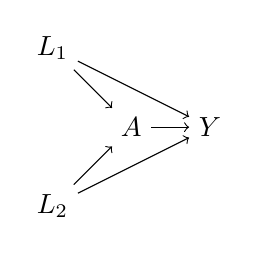
\begin{tikzpicture}
			% nodes
			\node (L1) at (0, 2) {$L_1$};
			\node (L2) at (0, 0) {$L_2$};
			\node (A) at (1, 1) {$A$};
			\node (Y) at (2, 1) {$Y$};
			% edges
			\draw[->]
				(L1)	edge (A)
				(L2)	edge (A)
				(L1)	edge (Y)
				(L2)	edge (Y)
				(A)	edge (Y);
		\end{tikzpicture}
	\end{center}

\noindent The above diagram is a representation of a mathematical {\it graph}: a collection of nodes and edges. We can define the relative position of nodes (the easy part), whereupon \LaTeX{} will output their position absolutely on our document (the hard part). Again, while the syntax appears tedious at first, we quickly see how powerful this tool is in making professional-looking output. Now let's consider a much more involved diagram, just for fun!

	\tikzstyle{block}	= [rectangle, draw, text width = 5em, text centered, rounded corners, minimum height = 3em]
	\tikzstyle{line}	= [draw, -latex]

	\begin{center}
		\scalebox{0.6}{\begin{tikzpicture}[node distance = 5cm, auto]
    			% place nodes
    			\node [block] (gen) {Data Generation};
			\node [block, right of = gen] (init) {Sample i};
			\node [block, above right of = init] (psm0) {PSM};
			\node [block, below right of = init] (bootc) {Bootstrap};
			\node [block, above right of = psm0] (base) {$\hat{\sigma}_\beta^2$};
			\node [block, below right of = psm0] (boots) {Bootstrap};
			\node [block, right of = bootc] (sampc1) {Unmatched Sample 1};
			\node [block, below of = sampc1, yshift = 2.95cm] (sampc2) {Unmatched Sample 2};
			\node [block, below of = sampc2, yshift = 2.95cm] (sampc3) {Unmatched Sample $m_{\text{b}}$};
			\node [block, right of = boots] (samps1) {Matched Sample $m_{\text{b}}$};
			\node [block, above of = samps1, yshift = -2.95cm] (samps2) {Matched Sample 2};
			\node [block, above of = samps2, yshift = -2.95cm] (samps3) {Matched Sample 1};
			\node [block, right of = samps2] (simp) {$\hat{\sigma}_\beta^2$};
			\node [block, right of = sampc1] (psm1) {PSM};
			\node [block, right of = sampc2] (psm2) {PSM};
			\node [block, right of = sampc3] (psm3) {PSM};
			\node [block, right of = psm2] (comp) {$\hat{\sigma}_\beta^2$};
			% draw edges
			\path [line] (gen) -- (init);
			\path [line] (init) -- (psm0);
			\path [line] (init) -- node {Complex}(bootc);
			\path [line] (psm0) -- node {Baseline}(base);
			\path [line] (psm0) -- node {Simple}(boots);
			\path [line] (boots) -- (samps1);
			\path [line] (boots) -- (samps2);
			\path [line] (boots) -- (samps3);
			\path [line] (bootc) -- (sampc1);
			\path [line] (bootc) -- (sampc2);
			\path [line] (bootc) -- (sampc3);
			\path [line] (sampc1) -- (psm1);
			\path [line] (sampc2) -- (psm2);
			\path [line] (sampc3) -- (psm3);
			\path [line] (samps1) -- (simp);
			\path [line] (samps2) -- (simp);
			\path [line] (samps3) -- (simp);
			\path [line] (psm1) -- (comp);
			\path [line] (psm2) -- (comp);
			\path [line] (psm3) -- (comp);
			% draw circle
			\node [yshift = -2.50cm, xshift = 2.25cm] (text) {$i \in \{ 1, \ldots, m_{\text{s}} \}$};
			\draw[black, ->] (text) + (80:2.25cm) arc(80:-260:1cm);
		\end{tikzpicture}}
	\end{center}

\subsection{Creating Graphs with the Tikzpicture Environment}

The pgfplots package extends the TikZ package to make creating plots of functions a breeze.

	\begin{center}
		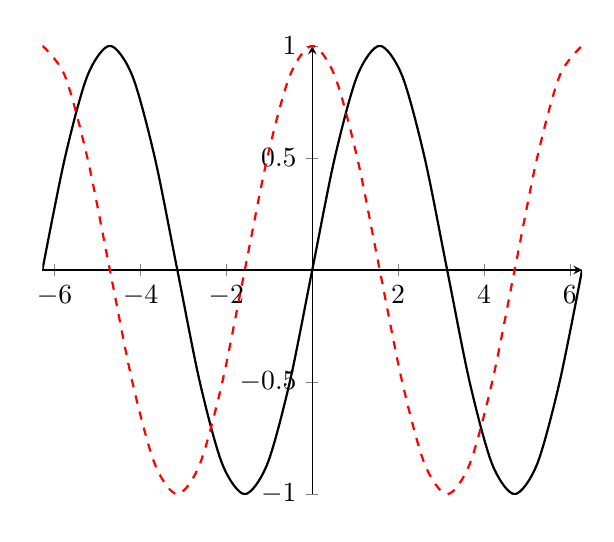
\begin{tikzpicture}
			\begin{axis} [axis lines = center, ymin = -1, ymax = 1]
				\addplot [domain = -2*pi:2*pi, smooth, thick] { sin(deg(x)) };
				\addplot [domain = -2*pi:2*pi, smooth, thick, red, dashed] { cos(deg(x)) };
			\end{axis}
		\end{tikzpicture}
	\end{center}

\noindent Above, we have plotted familiar sine and cosine functions over a manually specified domain. The syntax is much cleaner than that of the base version of the tikzpicture environment. By restricting our domain with an \verb!\addplot! call, we can also write piecewise functions, as shown below.

	\begin{center}
		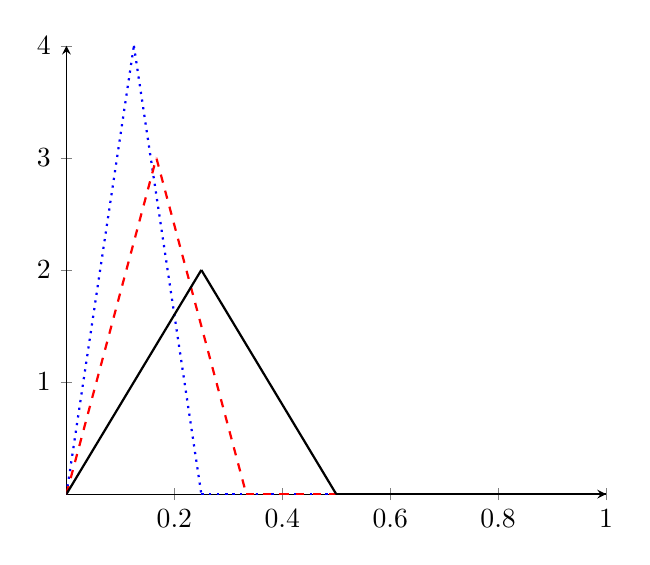
\begin{tikzpicture}
			\begin{axis} [axis lines = center]
				\addplot [domain = 0.000:0.125, smooth, thick, blue, dotted] { 32 * x };
				\addplot [domain = 0.125:0.250, smooth, thick, blue, dotted] { 8 - 32 * x };
				\addplot [domain = 0.250:1.000, smooth, thick, blue, dotted] { 0 };
				\addplot [domain = 0.000:0.167, smooth, thick, red, dashed] { 18 * x };
				\addplot [domain = 0.167:0.333, smooth, thick, red, dashed] { 6 - 18 * x };
				\addplot [domain = 0.333:1.000, smooth, thick, red, dashed] { 0 };
				\addplot [domain = 0.000:0.250, smooth, thick] { 8 * x };
				\addplot [domain = 0.250:0.500, smooth, thick] { 4 - 8 * x };
				\addplot [domain = 0.500:1.000, smooth, thick] { 0 };
			\end{axis}
		\end{tikzpicture}
	\end{center}

\noindent This is by no means an exhaustive characterization of visualizations that you can make in \LaTeX{}! As mentioned earlier, there are hundreds of templates available online to help you get started. Again, this is one of the more technical aspects of this program, so go slow and always read your error messages!

\end{document}